\documentclass[10pt,letterpaper]{article}
\usepackage[T1]{fontenc}
\usepackage{iftex}
\ifPDFTeX\usepackage[utf8]{inputenc}\fi
\usepackage{lmodern,microtype}
\usepackage[margin=0.95in]{geometry}
\usepackage{amsmath,amssymb,amsthm,booktabs,tabularx,array,graphicx}
\usepackage[round,authoryear]{natbib}
\usepackage[dvipsnames]{xcolor}
\usepackage{enumitem}
\usepackage{caption}
\usepackage{placeins}
\usepackage[colorlinks=true,allcolors=MidnightBlue,breaklinks=true]{hyperref}
\usepackage{xurl}
\graphicspath{{../figures/}}
\newcommand{\E}{\mathbb{E}}
\newcommand{\Prb}{\mathbb{P}}
\newcommand{\ind}{\mathbf{1}}
\newcommand{\R}{\mathbb{R}}
\newcommand{\gate}{\mathrm{gate}}
\newcommand{\eager}{\mathrm{eager}}
\newtheorem{proposition}{Proposition}
\newtheorem{lemma}{Lemma}
\newtheorem{definition}{Definition}
\setlist{nosep,leftmargin=*}
\captionsetup{font=small,labelfont=bf}
\setlength{\parskip}{3pt}
\setlength{\parindent}{1em}
\setlength{\emergencystretch}{2em}
\title{What Should Reference Labels Buy?\\Estimation, Certification, and Repair\\in Conjunctive Evaluations}
\author{Xu Chen\\\small\texttt{xchen992@gatech.edu}}
\date{October 10, 2026}
\hypersetup{pdftitle={What Should Reference Labels Buy?},pdfauthor={Xu Chen},pdfsubject={Reference checking in conjunctive evaluation}}
\begin{document}
\maketitle
\begin{abstract}
When a rubric task passes only if every criterion passes, checking an LLM judge against reference labels serves three goals: estimating accuracy, certifying outcomes, and repairing verdicts. We find that these gains can diverge sharply. In JudgmentBench, checking all 4,316 criteria on which two judges disagree corrects 1,217 criterion errors, yet immediate updating increases task disagreements from 244 to 245. To understand this outcome, we hold queried labels fixed and derive an exact accounting of new false passes prevented by certificate-gated updating and repairs delayed until certification. Under disagreement-first continuation, delayed repairs dominate the intermediate- and high-budget JudgmentBench comparison; at an 84\% budget, the penalty is 6.0 or 3.9 disagreements per 100 matched outputs under two reference panels. Allocation has a different tradeoff: at a 20\% budget, mixing certification with random sampling increases certification in all nine analysis cells, but repair gains are much larger in JudgmentBench than in RuVerBench. We trace this difference to which verdicts receive certificates and which repairs occur before certification. Finally, configurations with identical criterion confusion counts favor opposite update rules, showing why task associations are needed to plan verification. Together, these results connect a checking budget to the particular evaluation claim it should support.
\end{abstract}

\section{Introduction}
Rubric-based evaluation breaks a complex output into several judgments. A model may satisfy a requested format, include the necessary evidence, and avoid a prohibited error. An evaluator then combines these judgments into a score or verdict. When success requires every retained condition to hold, one failed condition determines the outcome. APEX-Agents provides a practical example: its task-level Pass@1 requires all criteria to be satisfied \citep{vidgen2026apex}. We observe a striking consequence in JudgmentBench: checking all 4,316 criteria on which GPT-5.4 and GPT-5.4-mini disagree corrects 1,217 criterion errors, yet task disagreements rise from 244 to 245. Four verdicts are repaired, but five correct rejections become false passes. The checks remove the judge's reasons for rejecting those outputs without reaching the criteria that actually fail. This example motivates a task-level analysis of what reference checking accomplishes.

A limited checking budget introduces a second problem. The same reference label can contribute to estimating the judge's overall accuracy, certify a particular task, or change an existing verdict. A checked failure may certify a task that was already correctly rejected. Correcting a mistaken rejection may repair another task before its remaining conditions are checked. These are distinct uses of evidence. An allocation that produces more certificates can therefore leave fewer, the same number, or more incorrect verdicts than another allocation at the same cost.

Research on multi-predicate screening, Boolean-function evaluation, active testing, and prediction-assisted inference supplies tools for choosing and interpreting checks \citep{krivosheev2018hybrid,gkenosis2022sbfe,nguyen2018activetesting,angelopoulos2023ppi}. We study how their different objectives interact in rubric evaluation. Our design separates \emph{acquisition}, which chooses the labels to query, from \emph{updating}, which decides when to change a task verdict. Immediate updating substitutes every checked reference label and recomputes the conjunction. Certificate-gated updating changes the verdict only when the observed labels determine the whole task's outcome. Evaluating both rules on exactly the same acquired labels isolates the effect of the update rule.

We make two empirical contributions supported by exact accounting formulas. First, we connect task-level error configurations and query priorities to finite-budget update effects. We show how prevented false passes compete with delayed repairs, and find that the substantial high-budget delay in JudgmentBench survives the separately examined changes in reference and task composition; the small low-budget advantage is sensitive to those changes. Second, we trace allocation gains to certificates on initially correct and initially wrong verdicts, repairs made before certification, and newly introduced errors. This reveals why a fixed certification-plus-sampling allocation yields substantial repair gains in JudgmentBench but only small changes in RuVerBench. Our third research question tests the information needed for such comparisons: criterion summaries leave task associations unresolved, and restoring those associations narrows the conclusions compatible with the evidence.

The paper addresses three questions:
\begin{enumerate}[label=\textbf{RQ\arabic*.}]
\item For the same queried reference labels, how do immediate and certificate-gated updates change task verdicts, and which error structures and query orders determine their budget-dependent effects?
\item How do sampling units and query allocations trade estimation precision against certification coverage and verdict repair, and when do certification gains translate into fewer residual disagreements?
\item Which task-level conclusions are determined by criterion summaries and queried reference labels, what additional task associations are needed, and how does identification differ from statistical estimation?
\end{enumerate}
Our evidence is a retrospective replay of released labels and saved judge predictions. We use those labels as specified references, and separately examine how changing the human reference changes the findings. This permits controlled comparisons without treating every recorded disagreement as an adjudicated judge error.

\section{Setting and study design}\label{sec:setting}
\subsection{Four evaluation targets}
An evaluation frame contains $N$ units. Unit $i$ has $k_i$ retained criteria, with binary reference labels $Y_{ij}$ and judge predictions $P_{ij}$; one denotes PASS. Write $M=\sum_i k_i$, $Z_i=\prod_jY_{ij}$, and $\widehat Z_i=\prod_jP_{ij}$. A unit is a task in RuVerBench and an output-by-rater annotation in the original JudgmentBench frame.

We distinguish criterion microaccuracy, $a=M^{-1}\sum_{ij}\ind(P_{ij}=Y_{ij})$; the aggregate task pass rate, $\theta=N^{-1}\sum_iZ_i$; individual certification, which determines a particular $Z_i$; and verdict repair, which reduces disagreement between reported verdicts and $Z_i$. The first two are population quantities, while the last two concern individual outcomes. Counting erroneous criteria found by a policy is a further diagnostic, not a substitute for any of these targets.

A query reveals one reference bit. The query controller sees predictions, metadata, and previously queried labels; it cannot inspect future references. Unless additional information is explicitly supplied, unqueried bits can take either value. In this query-only model, one observed FAIL certifies failure and observing every bit as PASS certifies success. Classical Boolean evaluation provides the foundations for these certificates \citep{gkenosis2022sbfe,unluyurt2004sequential}.

For a queried set $Q$, \emph{eager} updating replaces $P_{ij}$ by $Y_{ij}$ on $Q$ and recomputes the conjunction. \emph{Certificate-gated} updating retains $\widehat Z_i$ until $Q$ certifies an outcome, then reports that outcome. The gate therefore governs revisions; unresolved initial predictions remain visible. We count false passes (reported PASS, reference FAIL), false fails (reported FAIL, reference PASS), and their sum, denoted $E$.

\subsection{Data and constructed scoring targets}
RuVerBench supplies reference judgments on agentic coding (AC) and deep research (DR) criteria \citep{peng2026ruverbench}. We use saved predictions from four initial judge--domain runs and one additional GPT-5.4 low-reasoning DR run. We retain the predictions saved for these five study runs. The conjunction covers the criteria retained in the released frame after upstream filtering.

JudgmentBench provides rubric annotations for legal outputs and saved GPT-5.4 and GPT-5.4-mini scores \citep{yang2026judgmentbench}. Its native study concerns quality assessment by rubrics and preferences. We construct a strict all-pass target: every positive binary item must receive full credit, and every penalty occurrence count must be zero. The binary-only sensitivity removes penalty items. These choices define different success events. The original frame contains 1,539 annotations on 1,314 outputs from 30 base tasks, with 49 human raters. Table~\ref{tab:data} describes all nine analysis cells; cells sharing outputs are not independent replications.

\begin{table}[t]
\centering\small
\caption{Finite analysis frames. $N$ counts tasks in RuVerBench and output-by-rater annotations in JudgmentBench; $M$ counts criterion records. FP and FF compare the initial judge conjunction with the selected reference. The binary-only rows reuse the JudgmentBench annotations.}
\label{tab:data}
\begin{tabular}{lrrrrr}
\toprule
Frame / primary judge & $N$ & $M$ & Ref. PASS & FP & FF\\
\midrule
DR Gemini 3.1 Pro & 284 & 1,615 & 28 & 8 & 2\\
DR Qwen-plus & 284 & 1,615 & 28 & 28 & 3\\
DR GPT-5.4 low & 284 & 1,615 & 28 & 8 & 2\\
AC Qwen-plus & 210 & 843 & 117 & 31 & 10\\
AC DeepSeek v4-pro & 210 & 843 & 117 & 14 & 16\\
JB GPT-5.4, full & 1,539 & 23,487 & 227 & 24 & 220\\
JB GPT-5.4-mini, full & 1,539 & 23,487 & 227 & 36 & 223\\
JB GPT-5.4, binary-only & 1,539 & 20,229 & 266 & 181 & 67\\
JB GPT-5.4-mini, binary-only & 1,539 & 20,229 & 266 & 457 & 36\\
\bottomrule
\end{tabular}
\end{table}

The full JudgmentBench target exposes a pronounced error imbalance: GPT-5.4 predicts only 31 PASS verdicts, of which seven agree with a reference PASS. Removing penalties raises predicted passes to 380 and reference passes to 266. Of the 220 initial full-target false fails, 156 reject only penalty conditions and 64 reject both item types. This is a useful stress test for update delay. It also means that its effect sizes should be interpreted alongside the changed target and the other frames.

\subsection{Queries, budgets, and sensitivity designs}
The policy study compares seven acquisition rules: uniform criterion sampling; short circuit with natural, randomized, or judge-failure-first within-task order; disagreement-only checking; disagreement checking followed by random continuation; and disagreement-prioritized short circuit. A disagreement flag records any available auxiliary prediction that differs from the primary. Short-circuit policies stop a task after a queried FAIL or a completed PASS certificate. The disagreement-first continuation rule visits flagged criteria task by task, then samples globally from the remaining criteria. Within that first phase, task order determines which disagreements are reached first.

We evaluate 101 budget caps from zero to the entire criterion frame, three task orders, and 31 randomized priority realizations, with a separate canonical seed-0 realization. Task orders are release order, ascending predicted-failure count, and random. A stopped policy can spend less than its cap, so comparisons report actual queries. The focal 20\% allocation experiment compares criterion simple random sampling (SRS) with a fixed mix: up to half the budget goes to judge-first short circuit, followed by independent SRS from the unqueried remainder. The split is held fixed throughout the comparison.

Two additional designs examine stability. First, 206 repeatedly rated JudgmentBench outputs receive symmetric reference panels A and B, selected by an ID-hash rule. Both judge prediction vectors are held fixed. Crossed acquisition/evaluation references separate changing which labels are queried from re-reading the same query positions under another reference. Second, 399 whole-base-task resamples retain complete output, rater, and criterion blocks. Each replicate recalculates frame size and budget and reruns acquisition. Query-order variation, reference variation, and task-composition variation are reported separately. Appendices~\ref{app:expectations}--\ref{app:disclosure} provide the formulas, sampling procedures, and reconstruction constraints.

\section{RQ1: How updating changes task verdicts}\label{sec:rq1}
\subsection{A repair can expose another error}
Consider a task with reference bits $(1,0)$ and judge bits $(0,1)$. Both conjunctions initially say FAIL. Checking the first criterion changes the eager bits to $(1,1)$, producing a false PASS. Gating retains FAIL because the unchecked second criterion could still fail. The partial correction removed the reason for the original rejection without discovering the actual failure.

Now consider reference bits $(1,1)$ with judge bits $(0,1)$. Checking the first criterion repairs the eager verdict, but gating waits for the second check before reporting PASS. The same query structure that prevents an exposed false pass can postpone a valid repair. The empirical question is which of these events occurs more often at a given budget.

Let $A_b$ count newly introduced false passes under eager updating and $D_b$ count initial false fails that eager has repaired while gating still lacks a certificate.
\begin{proposition}[Update accounting]\label{prop:update}
For a fixed reference and the same queried set under both update rules,
\begin{equation}\label{eq:balance}
E_b^{\gate}-E_b^{\eager}=D_b-A_b.
\end{equation}
\end{proposition}
Partitioning tasks by their initial and reference verdicts proves the identity (Appendix~\ref{app:events}). The net effect depends on when erroneous rejections are corrected and actual failures are discovered. Their positions within each task and the query order determine the length of that interval.

For uniform sampling of $m$ criteria, an event requiring $r$ particular bits to be observed and $f$ other bits to remain unobserved has probability
\begin{equation}\label{eq:event}
h(M,m;r,f)=\frac{\binom{M-r-f}{m-r}}{\binom{M}{m}},
\end{equation}
with infeasible combinations assigned zero. For a susceptible initially correct FAIL, all predicted failures must be queried while every reference failure remains unqueried. For an initial false FAIL, delayed repair requires querying all predicted failures without completing the rubric. Summing these task events gives $\E[A_b]$ and $\E[D_b]$. Applying the same calculation within the active priority group gives exact expectations for disagreement-first continuation. The calculation is exact for the fixed reference and integrates over query randomization while retaining the observed dependence among criterion errors.

\subsection{Delayed repairs dominate the high-budget JudgmentBench comparison}
Under disagreement-first continuation, we find that delayed repairs dominate the high-budget JudgmentBench comparison (Table~\ref{tab:update}). The table separates analytical expectations from means over 31 query orders. In full JudgmentBench at a 20\% cap, the expected prevention of new false passes slightly exceeds delayed repair. At 84\%, the expected delay reaches 108.2 annotations while prevention remains 11.9. The net penalty is 96.3 disagreements. Both update rules converge to the reference at complete observation, so the penalty eventually returns to zero.

\begin{table}[t]
\centering\small
\caption{Matched-query updating under disagreement-first continuation, release task order. Positive net differences mean more residual disagreements under gating. Expectations use the complete fixed reference; the last column averages 31 saved query orders. Counts refer to annotations, not independent base tasks.}
\label{tab:update}
\begin{tabular}{llrrrrr}
\toprule
JB GPT-5.4 target & Cap & Queries & $\E[A_b]$ & $\E[D_b]$ & $\E[D_b-A_b]$ & Order mean\\
\midrule
Full & 20\% & 4,697 & 7.1 & 5.2 & $-2.0$ & $-2.1$\\
Full & 84\% & 19,729 & 11.9 & 108.2 & $+96.3$ & $+97.6$\\
Binary-only & 20\% & 4,046 & 28.2 & 36.4 & $+8.2$ & $+8.3$\\
\bottomrule
\end{tabular}
\end{table}

The task structure explains why the effect depends on the target. Full JudgmentBench has many initial false fails whose erroneous rejections can be corrected well before all passing conditions are checked. Binary-only has fewer false fails and many more initial false passes. Changing the target also changes rubric lengths, priorities, and absolute budgets, so this comparison describes a joint change in evaluation design. In DR Gemini there are only two initial false fails, sharply limiting the possible repair backlog. Moreover, a task whose every criterion is predicted FAIL has no such window: correcting all its rejected criteria completes its certificate at the same time.

Acquisition order constrains the size of the update effect.
\begin{proposition}[Unresolved-task bound]\label{prop:serial}
Let $U(Q)$ count partly queried, uncertified units. With the same fixed reference and query set, $|E^{\gate}(Q)-E^{\eager}(Q)|\leq U(Q)$. A serial policy that certifies each task before starting the next has $U(Q)\leq1$ at every prefix.
\end{proposition}
Both rules agree on untouched and certified units, which proves the bound. Thus a large update effect requires checks dispersed across unfinished tasks. Figure~\ref{fig:budget} shows the complete-budget effects of disagreement-first continuation across three frames.

\begin{figure}[t]
\centering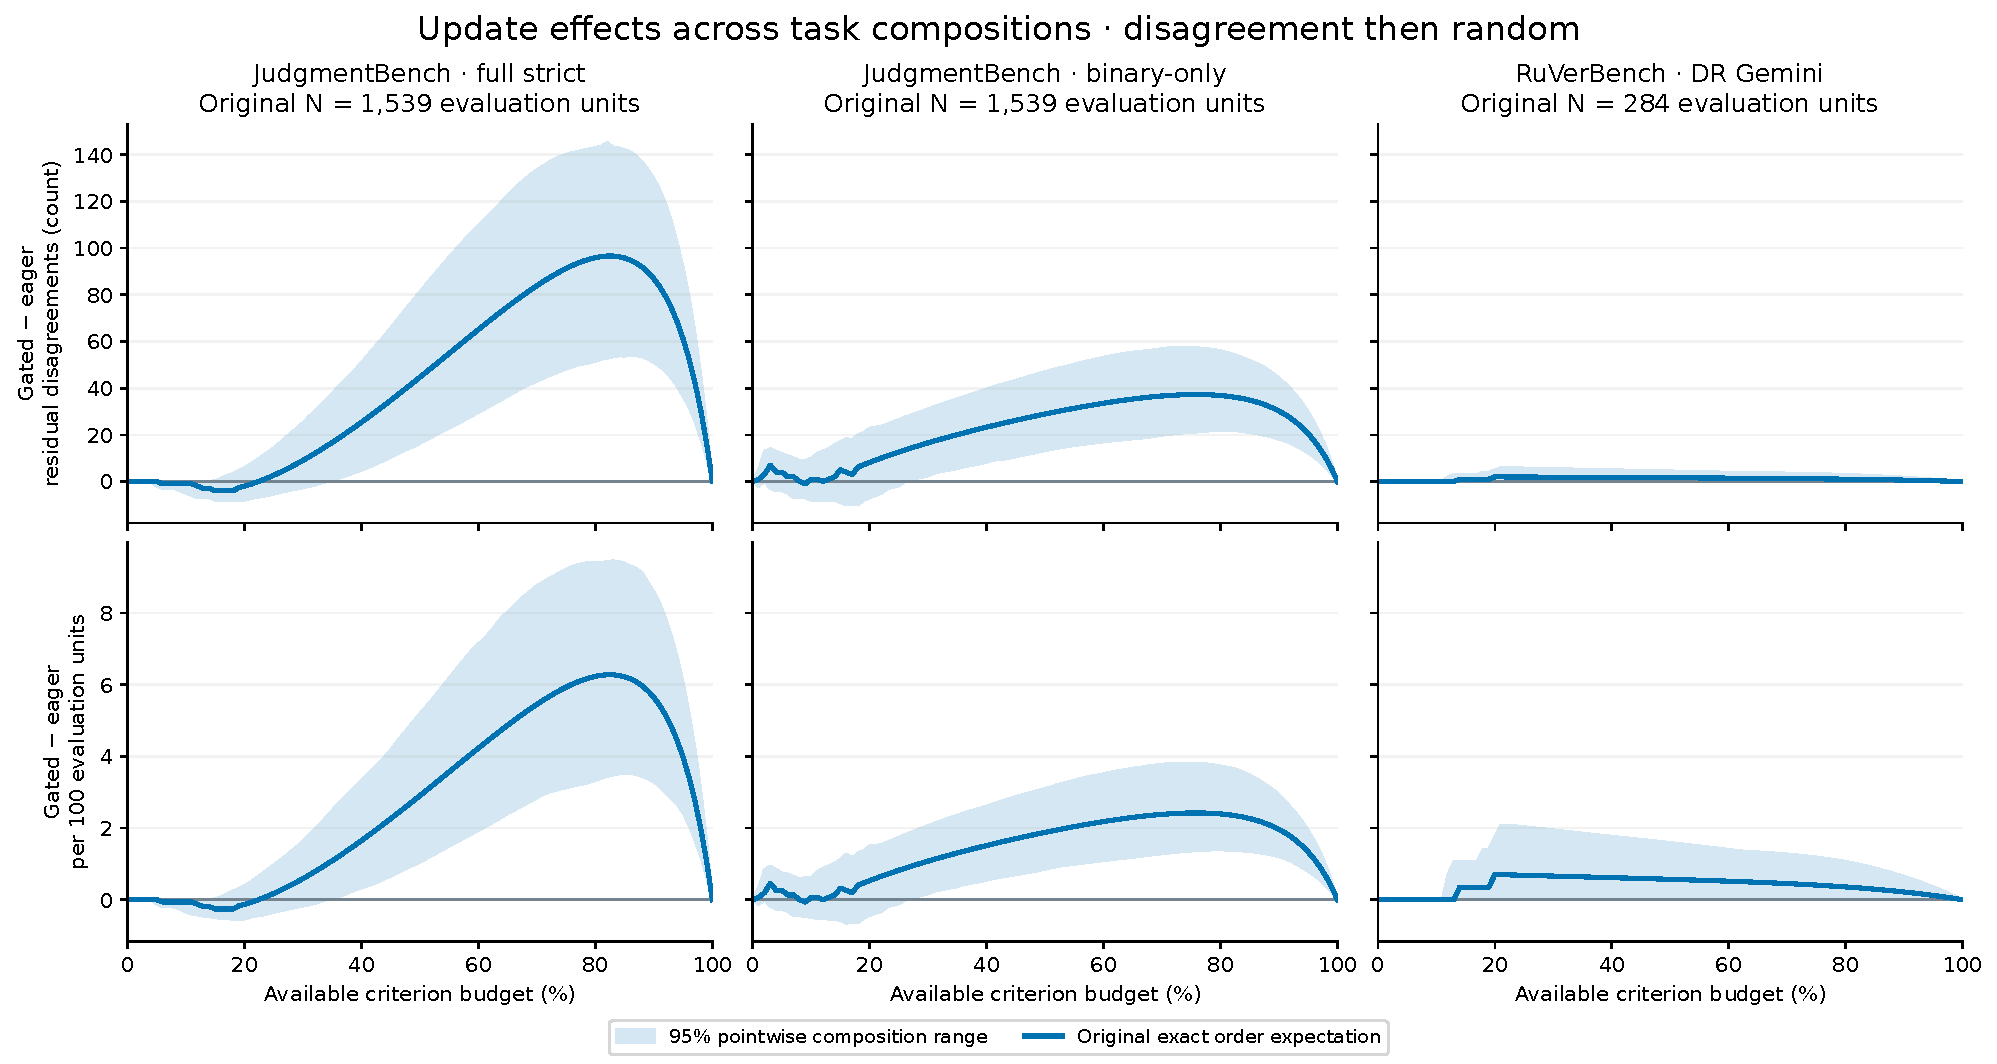
\includegraphics[width=\linewidth]{conjunction_robustness_budget.pdf}
\caption{Complete-budget update comparisons in full JudgmentBench, binary-only JudgmentBench, and DR Gemini. The plotted disagreement-first continuation policy uses release task order. Original effects are analytical expectations; the shaded pointwise ranges summarize 399 whole-base-task resamples. Each replicate reruns the policy at its recalculated budget. These ranges describe task-composition sensitivity, separately from query-order or reference-panel variation. Both endpoint effects are exactly zero.}
\label{fig:budget}
\end{figure}

\subsection{Which parts survive reference and composition changes?}
In full JudgmentBench, the expected 20\% contrast is $-0.13$ disagreements per 100 annotations, with a composition range of $[-0.54,0.39]$. At 84\%, it is $+6.26$, with range $[3.51,9.44]$. The small low-budget advantage is unstable; the high-budget repair delay persists across the examined compositions.

The separate matched-output analysis gives the same qualitative distinction. On 206 fixed outputs, the 84\% penalty is 6.0 or 3.9 disagreements per 100 outputs, depending on the reference panel. At 20\%, both panels instead give a small positive effect. Moving from the original annotation frame to this matched-output frame also changes weighting, sample composition, and the saved judge anchor; it is not a pure reference replacement. Within the matched frame, reference choice can reverse a comparison: binary-only uniform sampling at 20\% produces a mean difference of $+1$ under A and $-1$ under B.

These checks matter because the references themselves can disagree. In the repeated-annotation diagnostics, 32 of 54 initial false-fail annotations have another rater who also rejects the output, agreeing with the judge. Only 22 of 56 reference-PASS annotations are supported by every available peer rater. These are properties of the repeatedly rated subset, not estimates of which rater is correct. They motivate reporting the high-budget effect under both panels rather than treating the original 220 false fails as adjudicated model mistakes.

\section{RQ2: What additional certificates buy}\label{sec:rq2}
\subsection{A common-budget comparison}
We compare three uses of the same budget: random criterion sampling, a fixed certification-plus-sampling mix, and pure judge-first certification (Table~\ref{tab:allocation}). The mix increases certification and widens accuracy intervals in both focal frames. Pure certification produces still more resolved verdicts and fewer residual disagreements, but its adaptive queries do not supply the probability-sampling estimator used by the other two designs.

Across all nine cells, the mix increases certification in every paired query order. The mean change in residual disagreements ranges from about $-2.3$ to $+0.8$ across the five RuVerBench cells, compared with $-91.5$ to $-58.7$ across the four JudgmentBench cells. The focal DR Gemini comparison is the only positive mean contrast. The RuVerBench changes are small in absolute task counts. Below, we test task-composition sensitivity for the focal DR Gemini comparison and both strong-judge JudgmentBench targets.

\begin{table}[t]
\centering\small
\caption{Allocation at a 20\% criterion cap, release task order. Entries after queries are marginal medians across 31 orders. Width refers to a 95\% conditional hypergeometric interval for criterion microaccuracy. The mix spends up to half its cap on certification, then samples the remainder. Pure certification uses judge-first short circuit; the dash indicates that no probability-sampling accuracy interval is reported for it.}
\label{tab:allocation}
\begin{tabular}{llrrrr}
\toprule
Frame / primary & Allocation & Queries & Certified & Errors & Width (pp)\\
\midrule
DR Gemini & SRS & 323 & 131 & 8 & 5.5\\
& Fixed mix & 323 & 169 & 9 & 7.6\\
& Pure certification & 323 & 275 & 1 & ---\\
JB GPT-5.4, full & SRS & 4,697 & 798 & 223 & 2.2\\
& Fixed mix & 4,697 & 1,035 & 133 & 3.0\\
& Pure certification & 4,697 & 1,512 & 15 & ---\\
\bottomrule
\end{tabular}
\end{table}

We retain other acquisition controls to show that error discovery, certification, and repair can rank policies differently. At the DR 20\% cap, judge-first short circuit finds a median of 14 criterion errors and certifies 275 tasks; disagreement-first continuation finds 83 errors and certifies 160. Both leave a median of one task error. The opposing discovery and certification ranking holds in all 31 paired orders. It also occurs for the weaker JudgmentBench judge, but in none of the orders for the stronger judge. When a weaker judge uses a stronger judge to flag disagreements, evaluating that stronger judge as the primary provides a direct comparison with simply using its verdicts from the outset.

\subsection{Where the certificate gain goes}
Let $E_0$ be the initial verdict disagreement count, and let $C_W$ and $C_R$ count certified units that were initially wrong and right. As in Proposition~\ref{prop:update}, $D$ counts repairs made before certification and $A$ counts introduced false passes.
\begin{proposition}[Certification and repair accounting]\label{prop:allocation}
At every query endpoint,
\begin{equation}\label{eq:allocation}
C=C_R+C_W,\qquad E^{\eager}=E_0-C_W-D+A.
\end{equation}
\end{proposition}
Certified initially wrong units are repaired; among uncertified units, the only repairs and new errors are $D$ and $A$. For two allocations on the same frame,
\begin{equation}
\Delta C=\Delta C_R+\Delta C_W,\qquad
\Delta E^{\eager}=-\Delta C_W-\Delta D+\Delta A.
\end{equation}
A certificate on an already correct verdict adds evidence without repairing a mistake. Conversely, eager updating can repair a verdict before the task is certified. We use this distinction to locate the source of each allocation's gain.

In DR Gemini, the mix gains 40.0 certificates on average: 40.6 on initially correct tasks and $-0.6$ on initially wrong tasks. It also loses 0.2 uncertified repairs, leaving 0.8 more residual errors. The net certification gain therefore comes from verdicts that were already right. In JudgmentBench, certification increases by 237.7 overall and by 100.5 among initially wrong annotations. The mix loses 18.9 uncertified repairs but introduces 8.5 fewer new false passes, leaving 90.1 fewer disagreements. Figure~\ref{fig:allocation} displays the additive paired components.

\begin{figure}[t]
\centering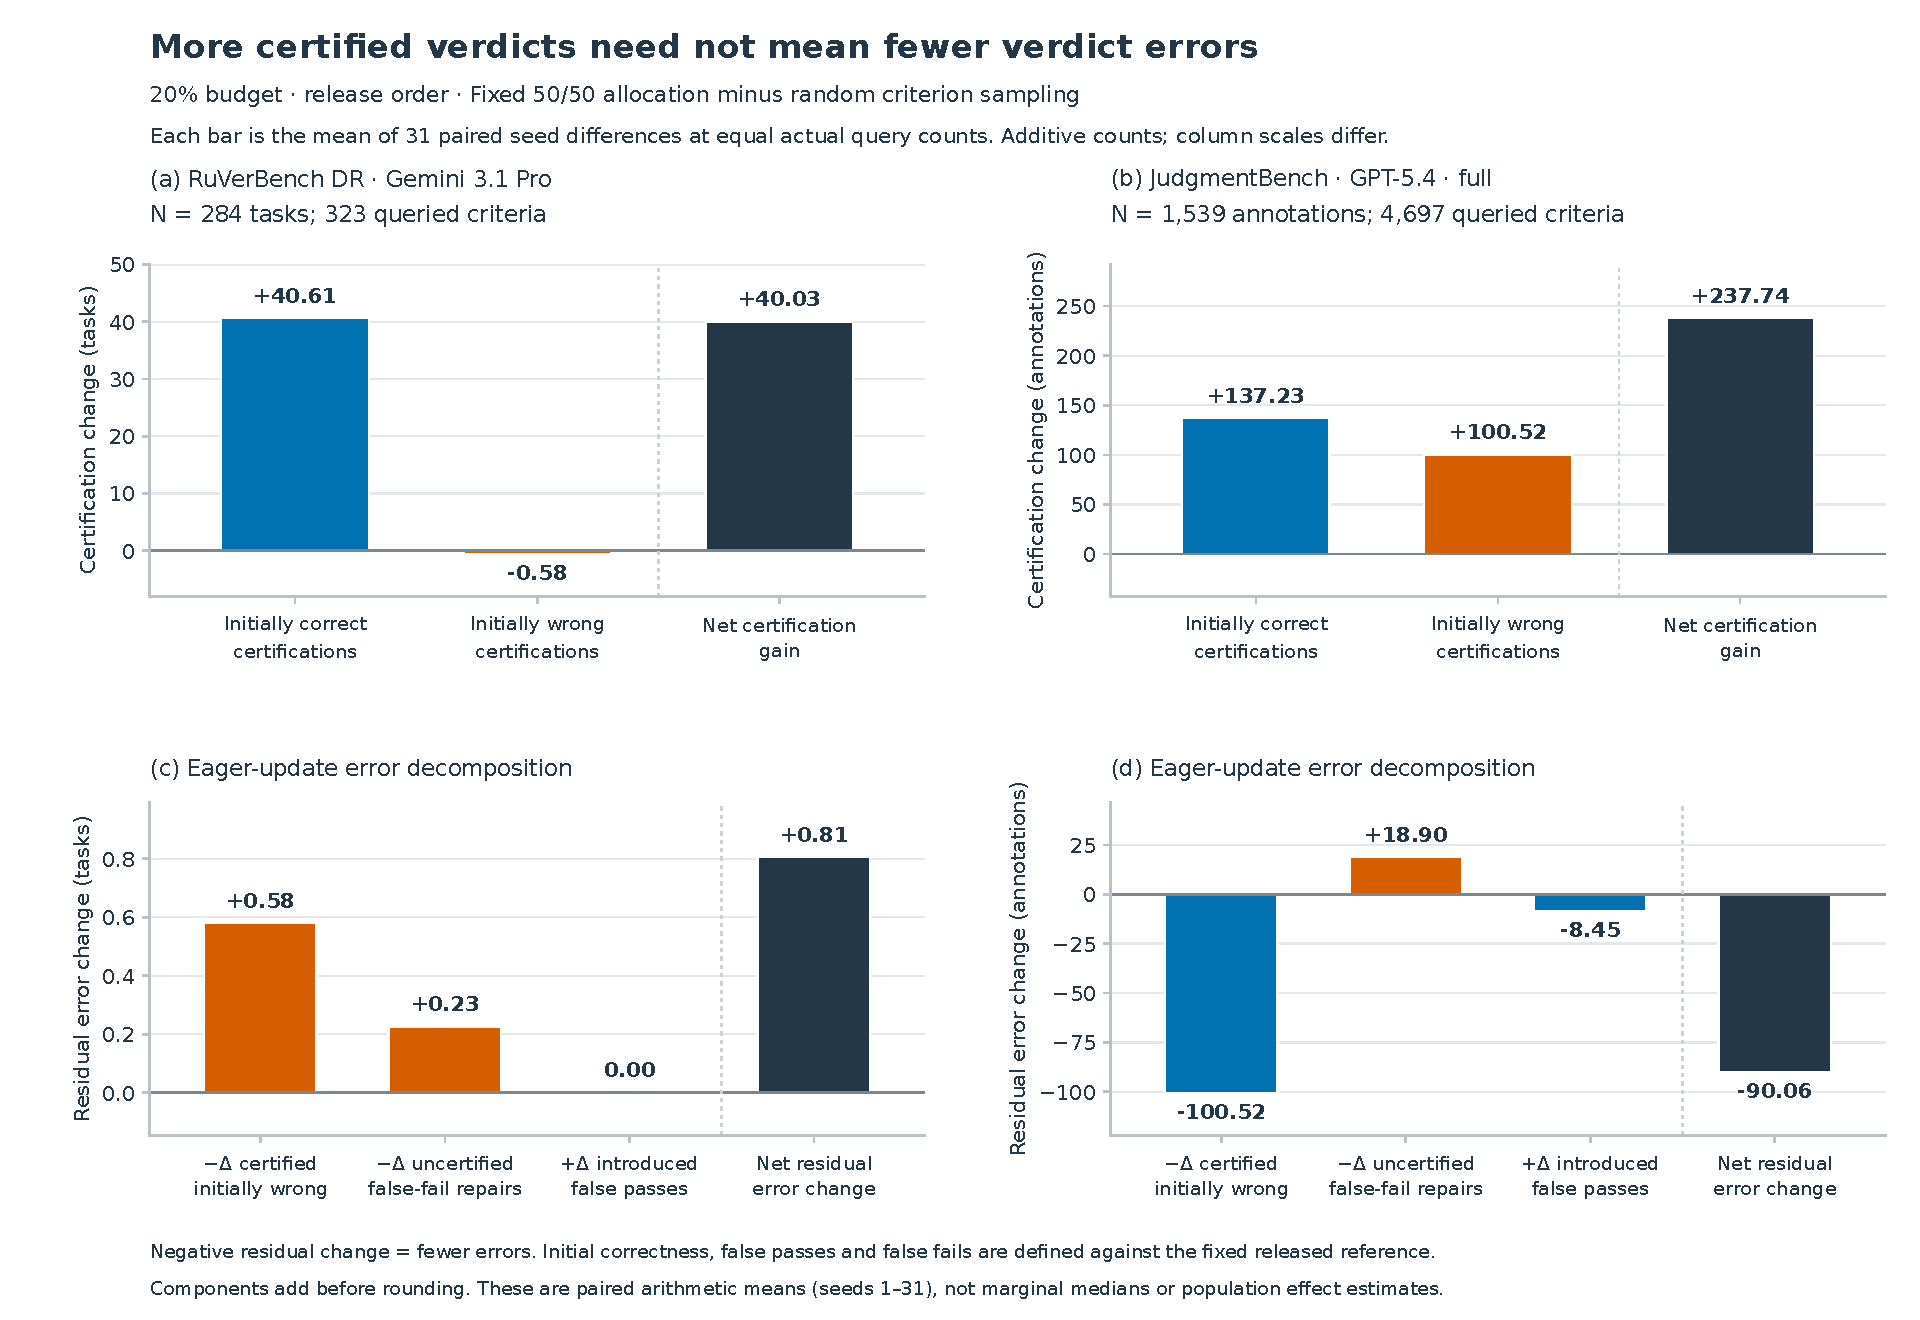
\includegraphics[width=0.96\linewidth]{conjunction_allocation_mechanism.pdf}
\caption{Allocation effects separated into where certificates are added and how residual disagreements change. Differences are fixed mix minus criterion SRS at a 20\% budget, release task order, averaged across 31 paired orders at equal query counts. The columns show DR Gemini (284 tasks, 323 queries) and full JB GPT-5.4 (1,539 annotations, 4,697 queries). Components add before rounding. The DR error increase describes the original frame; its direction varies in the task-composition analysis.}
\label{fig:allocation}
\end{figure}

The pattern persists differently under sensitivity checks. In JudgmentBench, both full and binary-only allocation comparisons reduce error in every one of the 399 task resamples. On the matched 206-output frame, all four acquisition/evaluation-reference combinations improve mean certification and repair at 620 queried labels. The matched-reference gains are $+27.6$ certificates and $-11.7$ disagreements under A, and $+32.1$ and $-8.7$ under B. Re-reading A's query positions under B gives $+14.9$ and $-4.5$; re-reading B's positions under A gives $+13.6$ and $-7.3$. A few individual orders in the crossed comparisons increase disagreement, even though their paired means improve.

DR gains certificates in every resample, but its repair contrast has 196 reductions, 198 increases, and five ties. We find stable certification gains in this DR Gemini comparison, while its small repair contrast changes with task composition.

\subsection{Preserving estimation while targeting certification}
The fixed mix also provides a transparent sampling estimator. If its first phase observes set $C$, the remainder contains $R=M-|C|$ bits. Draw $n$ of those bits by SRS and write $S$ for the sample. With $a_u=\ind(P_u=Y_u)$,
\begin{equation}\label{eq:estimator}
\widehat a=\frac{\sum_{u\in C}a_u+(R/n)\sum_{u\in S}a_u}{M}.
\end{equation}
Conditional on the first phase, this estimator is unbiased because the second phase is an independent probability sample. We invert hypergeometric tails for the unknown remainder agreement count and add the known first-phase total. This yields a fixed-budget conditional interval. Its justification follows from the design, in the tradition of finite-population sampling \citep{horvitz1952generalization}, rather than from the observed coverage in 31 repeats.

Alongside SRS, we compare proportional stratification and pilot-based Neyman allocation using primary predicted PASS/FAIL strata. Pilot labels count toward the budget. Known pilot totals are added to estimated remaining stratum totals; hypergeometric count bounds are combined with Bonferroni error allocation. These controls isolate a conventional design-based alternative alongside the prediction-powered methods developed in prior work \citep{angelopoulos2023ppi,fisch2024stratppi,kim2026humanreviews}.

Conservative interval width and empirical precision tell different stories. At the full-JudgmentBench 20\% cap, mean guaranteed widths are 2.21 pp for SRS, 3.47 for proportional stratification, and 3.74 for pilot Neyman. Yet proportional stratification reduces empirical RMSE in AC DeepSeek from 2.35 to 1.40 pp and in DR Gemini from 1.37 to 1.19 pp. Full JudgmentBench instead changes from 0.50 to 0.57 pp. Figure~\ref{fig:estimation} reports both width and RMSE for all nine cells, retaining improvements and contrary outcomes.

Estimating $\theta$ calls for another sampling unit. Select a fixed SRS of tasks and certify their outcomes, either by reading every rubric item or by stopping at the first failure. Both procedures observe the same sampled $Z_i$ and give the same pass-rate estimator. For 57 sampled DR tasks, median query cost falls from 319 to 67; for 308 JudgmentBench annotations, it falls from 4,690 to 1,002. Their exact design RMSEs for task pass rate are 3.54 and 1.81 pp. This fixed-unit-count design has variable label cost; it answers a different resource question from Table~\ref{tab:allocation}.

\section{RQ3: What criterion summaries leave unresolved}\label{sec:rq3}
The update mechanism depends on which failures co-occur within a task and where they lie in the query order. Criterion confusion counts do not retain these associations. We test their sufficiency by shuffling references within task-length $\times$ primary-prediction $\times$ criterion-category strata, preserving the stratum confusion counts, task lengths, predictions, and observable priorities.

Across 64 such configurations, the full-JudgmentBench uniform-sampling effect at 20\% changes from $+12.25$ disagreements in the original frame to values between $-9.76$ and $-1.48$. We observe the opposite preferred update rule under equal error costs in every configuration, despite identical criterion summaries. Across the nine cells, two policies, and five caps, 44 of 90 conditions admit an opposite-sign effect. These are counterexamples to information sufficiency, not estimates of a reversal frequency in new settings. With every stratum's confusion counts preserved, reference passes fall from 227 to between 108 and 132 across these 64 configurations. These changes jointly alter task success and error structure; our comparison tests the sufficiency of the summaries.

We next hold the reference frame fixed and vary what information is disclosed. In the query-only model, let $n_P$ and $n_F$ denote certified PASS and FAIL counts. Unrestricted completions give the sharp endpoint range
\begin{equation}\label{eq:bounds}
\theta\in\left[\frac{n_P}{N},1-\frac{n_F}{N}\right].
\end{equation}
Each unresolved task can independently be completed to PASS or FAIL, so the endpoints are attainable. More certificates narrow this range. A probability sample can nevertheless give a useful statistical estimate of $\theta$ while many individual tasks remain unresolved: logical identification and sampling precision answer different questions \citep{rao2026agreement,chen2026partial}.

Additional trusted summaries change the feasible set. Our disclosure replay begins with reference-containing confusion margins grouped by task length and prediction, refines them by criterion category, and then restores labels linked to whole tasks. Binary mixed-integer optimization computes attainable minimum and maximum pass totals. For DR Gemini, the initial margins leave the pass rate between 4.23\% and 16.90\%, a width of 12.68 pp. These margins comprise 38 disclosed count cells, not 38 new reference queries. Full link restoration recovers the observed pass rate.

Appendix~\ref{app:disclosure} gives a complete two-task example of how a trusted total and linked observations jointly identify the pass rate. Aggregate identification can still leave individual verdicts unresolved.

The practical implication is to report the information that supports the intended conclusion. Linked criterion records support analysis of update and certification behavior; criterion-level confusion summaries alone generally do not. RuVerBench already releases linked records, which make this replay possible. Preserving these links in downstream validation reports lets evaluators examine consequences that aggregate agreement conceals.

\section{Related work}\label{sec:related}
Multi-predicate screening studies condition-level crowd queries, posterior stopping, and downstream classification loss \citep{krivosheev2018hybrid,krivosheev2018screening,krivosheev2020active}. Sequential system testing and stochastic Boolean-function evaluation formalize how costly component checks determine an outcome \citep{unluyurt2004sequential,gkenosis2022sbfe,ghuge2026certification}. Structured agent evaluation also uses node-level checks and short circuit \citep{gou2025mind2web2}. Our logical certificates use these foundations. The empirical extension is to compare their role in repairing an already available judge verdict on matched queried sets.

Selective correction and local error propagation have close precedents. ActiveClean separates sample selection from model updating and shows why mixed clean and dirty data can distort learning \citep{krishnan2016activeclean}. Query-Guided Verification traces AND/OR query provenance, including cases where lowering a component's error probability raises a worst-case output score \citep{schreiber2026queryguided}. Its maximum-error score uses independent verification errors and differs from our realized FP/FF counts after exact bit replacement. Correction-and-corruption analysis also compares selective and unconditional application on fixed candidates and selects applications using estimated correction and corruption rates \citep{reitich2026correction}. Our contribution rests on the event decomposition, quantified budget curves, and their observed stability in rubric frames, building on these correction principles.

Failure discovery and performance estimation have long motivated different sample choices. DeepEST combines failure-oriented selection with population estimation, while recent multi-objective test selection compares discovery, estimation, and retraining \citep{guerriero2021deepest,zhang2026testselection}. Active Testing and prediction-assisted inference use partial trusted labels to estimate aggregate performance \citep{nguyen2018activetesting,chaganty2018price,angelopoulos2023ppi}. StratPPI studies stratified allocation, and Kim uses a two-phase doubly robust design and pilot information to plan human-review requirements \citep{fisch2024stratppi,kim2026humanreviews}. We add the joint accounting of certification and verdict repair, while using conventional sampling controls for estimation.

Different guarantees govern different decisions. Trust or Escalate calibrates acceptance and escalation of pairwise judgments to control disagreement risk among accepted judgments under its calibration assumptions \citep{jung2025trust}; audit-efficient best-agent identification targets system selection \citep{ao2026audits}. A logical certificate instead resolves a particular conjunction from observed reference bits. Evaluation-protocol and partial-identification work further distinguishes the conclusions licensed by aggregated information \citep{rao2026agreement,chen2026partial}.

Finally, human uncertainty affects automatic-evaluator assessment \citep{elangovan2025uncertainty}. Physician disagreement in HealthBench has been studied through variance decomposition and prediction \citep{borgohain2026disagreement}. Our reference sensitivity carries this concern through the checking protocol: it fixes both judges, changes the reference panel, and separates re-reading a fixed query set from rerunning acquisition. The resulting differences concern protocol conclusions as well as initial agreement.

\section{Discussion and limitations}\label{sec:limits}
Our comparisons suggest three practical choices. For criterion accuracy, use probability sampling, with stratification or a certification phase when those serve the evaluation's goals. For individual certificates and logical pass-rate bounds, concentrate checks within tasks; judge-failure-first short circuit resolves many verdicts in the examined frames. For repair, choose an error tradeoff explicitly and consider how many tasks the acquisition policy leaves unfinished. A serial task-completing policy limits the eager--gated difference to one verdict, whereas dispersed checks can make the update rule consequential across many tasks.

For false-pass and false-fail costs $c_{FP}$ and $c_{FF}$, the expected gated-minus-eager loss is $c_{FF}\E[D]-c_{FP}\E[A]$. When $c_{FF}>0$ and $\E[A]>0$, gating has lower expected loss exactly when $c_{FP}/c_{FF}>\E[D]/\E[A]$. Using the unrounded expectations underlying Table~\ref{tab:update}, the break-even ratio is approximately 0.725 at a 20\% budget and 9.1 at 84\%. At the 84\% budget in this comparison, waiting for certificates pays off only when a false pass costs more than roughly nine false fails. These thresholds describe the saved frame. Prospective selection would require affordable estimates of the relevant error structures, a charged pilot budget, and confirmation on unused data.

The study has four limits. First, all repairs and certificates refer to released labels. We do not adjudicate the raters, and a rubric certificate does not establish complete occupational competence or correctness under requirements outside the rubric. Second, our all-pass targets are constructed from two data families. The large full-JudgmentBench update effect occurs in a FAIL-dominated judge regime; the binary-only and DR comparisons show how its magnitude changes. Third, the experiments are retrospective. Repeated query orders do not create new tasks, and resampling 30 curated base tasks assesses composition sensitivity without making them representative of every future environment. Reference and task-composition sensitivities are separate analyses, not a joint uncertainty interval. Fourth, query counts measure revealed bits, not expert time or money. They omit the cost of obtaining auxiliary predictions and resolving reference disagreement.

The complete-reference calculations are explanations of the observed frames. A new environment may have different task lengths, pass rates, error overlap, or query priorities. A useful extension would test a prespecified prediction of protocol performance on unused tasks or on a native all-pass benchmark. Such a study would address transfer of the mechanism; a claim about expert labor would additionally need measured annotation costs. The present paper supplies the decomposition and reproducible comparisons with which to formulate those tests.

\section{Conclusion}
A reference check can improve an estimate, establish an outcome, or repair a verdict, and these gains have different information requirements. Matched-query comparisons show that the cost of waiting for a certificate depends on the interval between correcting erroneous rejections and completing the task. Allocation comparisons show that additional certificates improve repair only through the tasks and error events they resolve. Reference and task-composition checks distinguish persistent effects from small, unstable contrasts. Reference labels should buy the evidence the evaluation needs: probability samples for population estimates, completed checks for individual certificates, and timely correction for verdict repair. Choosing among these objectives also means choosing where to query and when to update.

\section*{Data, code, and AI assistance}
Data, saved predictions, analysis code, figures, and manuscript build instructions are available at \url{https://github.com/Itsxuchen/RefEval}. Reproduction requires no model API calls. The package preserves upstream attribution and data terms and redistributes compact numerical records. JudgmentBench judge predictions are source-published; RuVerBench predictions come from our saved runs.

Codex and Claude assisted with code, analysis checks, literature searches, and drafting. We checked generated material against source papers, code, and saved data. The named human author is responsible for the manuscript.

\FloatBarrier
\begingroup
\small\raggedright
\bibliographystyle{plainnat}
\bibliography{paper_references}
\endgroup
\clearpage
\appendix
\section{Finite reference frames and verdict accounting}
\label{app:accounting}

Let $\mathcal J_i$ be the nonempty set of criterion slots for evaluation unit
$i$, with $k_i=|\mathcal J_i|$, $N$ units, and
$M=\sum_i k_i$ slots. Slots belong to exactly one unit. The released reference
and primary prediction for slot $u$ are $Y_u,P_u\in\{0,1\}$, where one denotes
PASS. Throughout this appendix they are fixed finite-population values. Define
\begin{equation}
 Z_i=\prod_{u\in\mathcal J_i}Y_u,
 \qquad \widehat Z_i^0=\prod_{u\in\mathcal J_i}P_u,
 \qquad \theta=\frac{1}{N}\sum_i Z_i.
 \label{app:eq:targets}
\end{equation}
Criterion microagreement is the distinct target
$a=M^{-1}\sum_u\mathbf 1\{Y_u=P_u\}$.
An error in the following equations means disagreement with this particular
reference. No equation identifies which of two disagreeing human raters is
substantively correct.

For JudgmentBench full strict, a positive binary item passes when its original
value is one, and a negative-weight occurrence-count item passes when its
original count is zero. The loader checks that their conjunction equals
attaining the rubric's maximum score. Binary-only retains positive binary
items and removes occurrence-count items. This changes both the success event
and the criterion population. The original unit is an output-by-rater
annotation; the alternative-reference analysis instead weights distinct
outputs equally. RuVerBench units use the criteria retained in its release.

\subsection{Certificates and update rules}
\label{app:certificates}

Let $Q\subseteq\bigcup_i\mathcal J_i$ be the queried slots and
$Q_i=Q\cap\mathcal J_i$. In the query-only information model, a FAIL
certificate is an observed reference failure, and a PASS certificate requires
observing every slot as PASS. Write
\begin{align}
 C_i^-&=\mathbf1\{\exists u\in Q_i:Y_u=0\},\\
 C_i^+&=\mathbf1\{Q_i=\mathcal J_i,\ Z_i=1\},
 \qquad C_i=C_i^-+C_i^+.
 \label{app:eq:certificates}
\end{align}
Eager updating substitutes every queried reference value immediately:
\begin{equation}
 \widehat Z_i^{E}(Q)
 =\prod_{u\in\mathcal J_i}
       \bigl(\mathbf1\{u\in Q\}Y_u+\mathbf1\{u\notin Q\}P_u\bigr).
 \label{app:eq:eager}
\end{equation}
Certificate-gated updating uses $Z_i$ once certified and otherwise retains
$\widehat Z_i^0$:
\begin{equation}
 \widehat Z_i^{G}(Q)=C_iZ_i+(1-C_i)\widehat Z_i^0.
 \label{app:eq:gated}
\end{equation}
Writing $Z_i$ here is shorthand for the value logically determined by a
certificate, not access to an unqueried reference. The implementation obtains
that value from the queried bits. Gating can retain an uncertified initial
PASS; it is not a protocol that publishes only certified outcomes.

\subsection{Acquisition implementations}
\label{app:acquisition}

The seven acquisition rules use a common slot map. Uniform criterion
sampling follows a global random priority. Three serial short-circuit rules
visit tasks in the stated order and visit their criteria in natural slot
order, random order, or predicted-FAIL-first order, respectively. They stop
the current task at its first observed reference failure or after completing
its rubric. Disagreement-only visits flagged criteria within each task and
stops after the flagged pool is exhausted; it can leave budget unused.
Disagreement-then-random uses that same flagged prefix, followed by a global
random ordering of all unflagged criteria. Disagreement-prioritized short
circuit visits, within a task, flagged slots first, then unflagged predicted
FAIL slots, then the remaining predicted PASS slots; its stopping rule is
the same serial certification rule.

For each DR primary, the auxiliaries are the other two saved DR judges
among Gemini 3.1 Pro, Qwen-plus and GPT-5.4 low. Each AC primary has the
other saved AC judge as its auxiliary: Qwen-plus or DeepSeek v4-pro.
JudgmentBench pairs GPT-5.4 with GPT-5.4-mini within the same scoring target.
The flag is the union of disagreements with available auxiliaries. Their
predictions are treated as available signals; their acquisition cost is not
included in the reference-bit budget.

The three task orders are release-relative order, ascending primary
predicted-failure count, and a random task order. Seeds 1--31 randomize ties
within the declared priorities. A separate canonical seed-zero realization
uses natural slot order for priority ties while retaining random priorities
for explicitly random policies and the random task order. Purpose-specific
streams derive from root seed 20260913, the replicate seed and a SHA256 hash
of the stream's name. Release-relative order refers to the loader's retained
unit ordering, not a randomized sample of deployment tasks. The analytical
mechanism calculations below hold this order fixed.

\subsection{Exact event decomposition}
\label{app:events}

Define predicted-failure slots $F_i=\{u\in\mathcal J_i:P_u=0\}$ and
reference-failure slots $T_i=\{u\in\mathcal J_i:Y_u=0\}$. An initially
correct FAIL is susceptible to a new false PASS only if $F_i$ and $T_i$ are
nonempty and disjoint. Its new-error event is
\begin{equation}
 A_i(Q)=\mathbf1\{F_i\ne\varnothing,\ T_i\ne\varnothing,
 F_i\cap T_i=\varnothing,\ F_i\subseteq Q,
 T_i\cap Q=\varnothing\}.
 \label{app:eq:introduced}
\end{equation}
An initially false FAIL has $T_i=\varnothing$ and
$F_i\ne\varnothing$. Eager updating repairs it once all its predicted
failures have been checked. Gating delays that repair until every criterion
has been checked. The delayed-repair event is therefore
\begin{equation}
 D_i(Q)=\mathbf1\{T_i=\varnothing,\ F_i\ne\varnothing,
 F_i\subseteq Q,\ \mathcal J_i\not\subseteq Q\}.
 \label{app:eq:delayed}
\end{equation}
Let $A(Q)=\sum_i A_i(Q)$, $D(Q)=\sum_i D_i(Q)$, and
$E_r(Q)=\sum_i\mathbf1\{\widehat Z_i^r(Q)\ne Z_i\}$ for
$r\in\{E,G\}$. Then
\begin{equation}
 E_G(Q)-E_E(Q)=D(Q)-A(Q).
 \label{app:eq:update-identity}
\end{equation}

\paragraph{Derivation.}
Initially correct PASS units have every prediction and reference equal to
one, so either update remains correct. An initially false PASS is repaired
exactly when a reference failure is queried, which also certifies FAIL; both
updates therefore agree. For an initially correct FAIL, an unqueried
predicted failure or a queried reference failure prevents eager PASS. Eager
can introduce a false PASS precisely in \eqref{app:eq:introduced}, while
gating retains the correct FAIL. For an initially false FAIL, the two rules
disagree precisely in \eqref{app:eq:delayed}. Summing these four exhaustive
initial classes proves \eqref{app:eq:update-identity}. In particular, correct
reference substitutions cannot introduce a false FAIL under conjunction.

If false PASS and false FAIL have fixed nonnegative costs $c_{\rm FP}$ and
$c_{\rm FF}$, their endpoint loss difference is
$c_{\rm FF}D-c_{\rm FP}A$. Thus equal-weight error comparisons are one
particular loss choice. Along a growing query transcript, gated error cannot
increase: every changed verdict is certified relative to the fixed
reference. Its difference from eager error can increase because eager may
repair false FAILs earlier. At zero queries and at a census the difference
is zero.

Both rules agree on untouched and certified units. If $U(Q)$ units have been
partially queried but remain uncertified, then
$|E_G(Q)-E_E(Q)|\leq U(Q)$. A serial short-circuit policy that completes or
certifies a task before starting the next has $U(Q)\leq1$ at every prefix.
This explains why changing the update rule has little room to change the
endpoint under that acquisition structure, even when dispersed querying has
a large effect.

\section{Finite-budget expectations over query order}
\label{app:expectations}

For uniform sampling of $h$ slots without replacement from a group of size
$G$, the probability of including $r$ specified slots and excluding $f$
other specified slots is
\begin{equation}
 H(G,h;r,f)=\frac{\binom{G-r-f}{h-r}}{\binom{G}{h}}.
 \label{app:eq:hypergeom-event}
\end{equation}
The specified inclusion and exclusion sets are disjoint. We set the
probability to zero when $r+f>G$, $r>h$, or $f>G-h$; in the empty case
$H(0,0;0,0)=1$. Equation~\eqref{app:eq:hypergeom-event} follows by choosing
the other $h-r$ observed slots from the $G-r-f$ unrestricted slots. It is a
sampling calculation and assumes no independence of reference errors.

For a uniform $m$-of-$M$ criterion query set, the two expectations are
\begin{align}
 \mathbb E[A(Q)]
 &=\sum_{i:\,F_i,T_i\ne\varnothing,\,F_i\cap T_i=\varnothing}
     H(M,m;|F_i|,|T_i|),\\
 \mathbb E[D(Q)]
 &=\sum_{i:\,T_i=\varnothing,\,F_i\ne\varnothing}
     \{H(M,m;|F_i|,0)-H(M,m;k_i,0)\}.
 \label{app:eq:uniform-expectations}
\end{align}
The complete-rubric event is contained in the event of observing every
predicted failure, which justifies the subtraction in the second line.
Linearity of expectation gives the expected update difference even though
events for different tasks are dependent under a fixed global budget.

\subsection{Prioritized groups}
\label{app:priority-groups}

The same calculation applies to a predetermined sequence of disjoint query
groups $\mathcal G_1,\ldots,\mathcal G_L$. Every slot in an earlier group is
queried before any slot in a later group, and order within each group is
uniformly random. At an interior cap $m$, let $\ell$ be the group satisfying
\[
 \sum_{g<\ell}|\mathcal G_g|\leq m
 <\sum_{g\leq\ell}|\mathcal G_g|,
 \qquad h=m-\sum_{g<\ell}|\mathcal G_g|.
\]
For a required set $R$ and forbidden set $S$, the event
$R\subseteq Q$, $S\cap Q=\varnothing$ has probability zero if a required
slot lies after $\ell$, a forbidden slot lies before $\ell$, or the two sets
overlap. Otherwise its probability is
\begin{equation}
 H\bigl(|\mathcal G_\ell|,h;
         |R\cap\mathcal G_\ell|,|S\cap\mathcal G_\ell|\bigr).
 \label{app:eq:group-event}
\end{equation}
At a complete group boundary, the next group has $h=0$. At a census the
event is determined directly by the complete query set. Substituting this
event probability for each term in
\eqref{app:eq:uniform-expectations} gives the grouped-order expectations.

For disagreement-then-random, a criterion is flagged when any available
auxiliary judge disagrees with the primary prediction. Each task's flagged
criteria form one group, tasks follow release order, and the final group
contains all unflagged criteria. The flagged tier is therefore not a single
global random sample. These groups depend on saved predictions and task
order, not hidden references. The analytical grid covers uniform criterion
and disagreement-then-random querying at 101 shares from zero to one. It
does not apply the predetermined-group formula to adaptive short-circuit
paths. Budget caps use the implementation's nearest-integer rule
$m=\operatorname{round}(bM)$, with ties to an even integer.

All expectations condition on the full reference, predictions and priority
groups. They explain the observed frames rather than provide a free
prospective policy selector. The 31 random-order means provide a Monte Carlo
check against these expectations; their standard error is the sample
standard deviation divided by $\sqrt{31}$, not uncertainty from sampling new
tasks.

\subsection{Matched-margin alternatives}
\label{app:permutations}

We construct 64 alternative assignments in each of nine analysis cells by
permuting reference labels within strata defined by task length, primary
prediction and criterion category or scoring mode. This preserves every
stratum's prediction/reference confusion counts, the task slots and lengths,
and all primary and auxiliary predictions. Root seed 20261007 and a
dataset-specific hash define the random streams. Both analytical policies
are evaluated at shares $0.05,0.20,0.50,0.84,0.95$, including originally
observed focal and peak regions. An alternative assignment with a different
update effect demonstrates that the retained summaries do not determine
that effect. These are retrospective counterexamples, not a null test for
random reference noise. The permutations can also change reference task
pass counts, initial task errors and their joint configuration, so they do
not isolate a causal effect of error correlation.

\section{Certification and repair under different allocations}
\label{app:allocation}

Let $E_0=\sum_i\mathbf1\{\widehat Z_i^0\ne Z_i\}$. For a query set $Q$,
write $C_W(Q)$ and $C_R(Q)$ for the numbers of certified units that were
initially wrong and initially right. Then
\begin{align}
 C(Q)&=C_W(Q)+C_R(Q),\\
 E_G(Q)&=E_0-C_W(Q),\\
 E_E(Q)&=E_0-C_W(Q)-D(Q)+A(Q).
 \label{app:eq:allocation-identity}
\end{align}
Every certified initially wrong unit is repaired under either rule. The
only further eager repairs are the uncertified false-FAIL repairs counted
by $D$, and its only new errors are those counted by $A$. This proves the
last two identities directly from the initial classes.

For two allocations applied to the same frame, define every signed
difference as mixed allocation minus uniform criterion sampling. Pairing
within a query-order replicate yields
\begin{equation}
 \Delta C=\Delta C_W+\Delta C_R,
 \qquad
 \Delta E_E=-\Delta C_W-\Delta D+\Delta A,
 \qquad
 \Delta E_G=-\Delta C_W.
 \label{app:eq:paired-allocation}
\end{equation}
We calculate these differences before averaging. Their means retain the
additive identities, whereas differences of marginal medians generally do
not. To describe where additional certificates go, we also report the
composition of the \emph{mixed-only} certified set, separately from the
uniform-only set. This gross composition remains meaningful when net
certification gain is zero or negative. More certificates on initially
correct units can provide useful confirmation without repairing an error;
it is not by itself evidence that an allocation is harmful.

The fixed mixed design spends up to $\lfloor m/2\rfloor$ labels on
judge-first serial short circuit, then draws a fresh uniform sample without
replacement from the remaining criterion slots. If short circuit completes
before its phase cap, the unused budget transfers to the random phase. All
revealed labels count toward the common actual total $m$. This contrasts
acquisition while the matched-query comparison in
Appendix~\ref{app:events} contrasts updating. Neither design uses hidden
initial-error classes to choose queries.

\section{Finite-population estimation and intervals}
\label{app:inference}

\subsection{An adaptive first phase followed by fresh sampling}

Set $a_u=\mathbf1\{P_u=Y_u\}$. Let the first-phase transcript reveal a set
$C$ of $c$ criterion labels with known correct count $t_C=\sum_{u\in C}a_u$.
Condition on that complete transcript. The remaining $R=M-c$ slots form a
fixed population. Draw an independent simple random sample $S$ of size $n$
without replacement from it, and observe $x=\sum_{u\in S}a_u$. For $n>0$,
\begin{equation}
 \widehat a=\frac{t_C+R x/n}{M},
 \qquad \mathbb E[\widehat a\mid C,\hbox{first-phase observations}]=a.
 \label{app:eq:conditional-estimator}
\end{equation}
The expectation follows from inclusion probability $n/R$ for every remaining
slot. Conditioning on the observed history accommodates the adaptive first
phase: the second-phase estimate expands only the unobserved remainder.
When $R=0$, the reference agreement is known exactly. When $R>0$ but $n=0$,
we report logical bounds $[t_C/M,(t_C+R)/M]$ and no design-unbiased point
estimate from this formula.

Let $S_R^2$ be the finite-population variance of the remainder's agreement
bits, with denominator $R-1$. For $R>1$ and $n>0$,
\begin{equation}
 \operatorname{Var}(\widehat a\mid\hbox{first phase})
 =\frac{R^2}{M^2}\left(1-\frac{n}{R}\right)\frac{S_R^2}{n}.
 \label{app:eq:fpc}
\end{equation}
The factor $1-n/R$ is the finite-population correction. Census remainders
have zero variance. Where a normal approximation is reported, $n\geq2$
permits the sample variance
$s^2=x(n-x)/[n(n-1)]$ to replace $S_R^2$. That approximation is evaluated
separately from the guaranteed intervals below.

\subsection{Inclusive hypergeometric inversion}
\label{app:hypergeom-ci}

For unknown remainder success count $K$, the sample count has probability
\begin{equation}
 \Pr_K(X=j)=\frac{\binom{K}{j}\binom{R-K}{n-j}}{\binom{R}{n}}.
 \label{app:eq:hg-pmf}
\end{equation}
Retain integer counts consistent with the sample and both inclusive tails:
\begin{equation}
 \mathcal K_\alpha(x)=
 \left\{K\in\{x,\ldots,R-n+x\}:
 \Pr_K(X\geq x)\geq\frac{\alpha}{2},\quad
 \Pr_K(X\leq x)\geq\frac{\alpha}{2}\right\}.
 \label{app:eq:hg-set}
\end{equation}
Let $K_L$ and $K_U$ be its minimum and maximum. The microagreement interval
is $[(t_C+K_L)/M,(t_C+K_U)/M]$. For every fixed true $K$, rejection by either
tail occurs with probability at most $\alpha/2$; a union bound gives coverage
at least $1-\alpha$. Discreteness can make it conservative. This is a
conditional, fixed-budget randomization guarantee with the reference held
fixed, not simultaneous coverage of every budget or validity under optional
stopping. At $n=0$ the count range is $[0,R]$, and at $n=R$ it is $[x,x]$.

The implementation compares ordinary tails numerically, but recomputes
near-threshold decisions using integer binomial coefficients and rational
$\alpha/2$. A tolerance triggers exact calculation rather than accepting an
endpoint. For example, with $R=16,n=2,x=0,\alpha=0.05$,
$K=13$ satisfies $\Pr(X=0)=\binom{3}{2}/\binom{16}{2}=0.025$ exactly and
must remain in the interval $[0,13]$. This resolves the floating-point
boundary case without altering the mathematical acceptance rule.

\subsection{Prediction strata and a charged pilot}
\label{app:strata}

Prediction strata are the nonempty sets with $P_u=0$ or $P_u=1$, known before
reference acquisition. Proportional allocation reserves one draw per
nonempty stratum when affordable, distributes remaining draws proportional
to stratum size, respects capacities, and resolves integer remainders by
descending fractional part with prediction-zero first on ties. Otherwise it
falls back to uniform sampling.

For the charged-pilot design, the initial allocation is
$\min(2,N_h)$ labels in stratum $h$. The design reserves at least one later
draw in each stratum not exhausted by that initial allocation. If the cap
cannot fund both stages, it falls back to uniform sampling. Otherwise the
pilot target is the larger of this minimum and $\lfloor0.2m\rfloor$, capped
to preserve the later draws. Additional pilot slots are allocated by stratum
size, leaving an unobserved slot in each initially noncensused stratum.
After pilot counts $p_h$ and observed agreement totals $t_h$, define
\[
 \widetilde a_h=\frac{t_h+1/2}{p_h+1},\qquad
 R_h=N_h-p_h,\qquad
 w_h=R_h\sqrt{\widetilde a_h(1-\widetilde a_h)}.
\]
The remaining budget is allocated by weights $w_h$, with a minimum of one
draw from each nonempty remainder and its capacity as an upper bound. The
same capacity-constrained proportional allocation and largest-remainder
rule determine integer counts. Pilot and remainder samples use separate
random-priority streams. All pilot labels are charged to the budget.

Conditional on the pilot, let the remainder sample in stratum $h$ have size
$n_h$ and agreement total $x_h$. Then
\begin{equation}
 \widehat a_{\rm strat}
 =\frac{\sum_h t_h+\sum_{h:R_h>0}R_hx_h/n_h}{M}
 \label{app:eq:strat-estimator}
\end{equation}
is conditionally unbiased. If $H$ strata are not censused, we obtain a count
interval in each at error level $\alpha/H$, sum their lower and upper bounds
and add the known pilot total. The union bound proves conditional coverage
at least $1-\alpha$ for the overall mean; independence between stratum
interval events is not required. Censused strata contribute their exact
counts. The accompanying normal approximation sums the variances in
\eqref{app:eq:fpc}, stratum by stratum, and clips endpoints to $[0,1]$.
It is unavailable when a noncensused stratum has fewer than two sampled
slots. These design-based controls are not an implementation of StratPPI.

At each of six shares $0.006,0.05,0.20,0.50,0.60,1$, we report bias, empirical
RMSE, coverage and interval width over 31 query-order replicates in each of
nine analysis cells. RMSE is
$[31^{-1}\sum_{s=1}^{31}(\widehat a_s-a)^2]^{1/2}$.
The replications describe the finite frames; coverage guarantees derive
from the sampling design and inversion, not the number of observed covered
replicates. Conservative simultaneous stratum bounds can be wider despite
a smaller empirical RMSE.

\subsection{Whole-task sampling}
\label{app:whole-task}

For estimating $\theta$, the separate whole-task panel fixes the number of
sampled evaluation units in advance and draws them uniformly without
replacement. Fully revealing an included unit and short-circuiting after
its first reference failure yield the same certified $Z_i$. Their sample
means and finite-population task-count intervals are consequently identical,
although their criterion-query costs differ. Here sample size is fixed and
label cost is random. This experiment is distinct from stopping task
sampling at a fixed label cap, which would generally alter inclusion
probabilities and require its own inference.

\section{Alternative references and task composition}
\label{app:sensitivity}

\subsection{Matched reference panels}
\label{app:reference}

The matched frame contains 206 outputs with at least two distinct raters.
The corresponding 431 annotations are distinguished from the original
1,539 annotation units. Outputs are sorted by base-task and output identity.
For each output, distinct-rater annotations are sorted by the SHA256 digest
of the literal string
\texttt{reference-panel-v1|output|rater|annotation}; the first two complete
rubric vectors form panels A and B. A separate ordering with salt
\texttt{judge-anchor-v1} chooses the annotation supplying the saved primary
and auxiliary predictions. The selection rule does not inspect label values
or agreement. Rubric-slot identities are checked before alignment, and the
same selections are used for both targets and both judges. A and B thus
refer to symmetric selections across outputs, not globally ranked raters or
a chronological improvement in reference quality.

Crossed comparisons distinguish the reference used for acquisition from
the reference used for reading and evaluating the resulting query set.
For acquisition panel $a\in\{A,B\}$, an adaptive policy obtains $Q^{(a)}$
using that panel's answers. For evaluation panel $e\in\{A,B\}$, queried
slots are re-read using $Y^{(e)}$, both updates are computed from those
answers, and residual disagreement is measured against the complete
$Y^{(e)}$. Off-diagonal comparisons therefore describe counterfactual
re-reading of fixed queried items. They do not retain panel A answers while
silently treating panel B as truth. Nonadaptive policies have identical
query sets for either acquisition panel. Adaptive short circuit can change
its stopping decisions and actual query count.

The update grid includes uniform criterion, disagreement-then-random and
judge-first short circuit at all 101 budget shares and seeds 1--31. The
allocation grid compares the mixed and uniform designs at the six shares
listed above, with equal actual query counts within each contrast. The four
crossed means share outputs and references and are not four independent
replications. Moving from the original frame to the matched frame also
changes composition, weighting and judge anchoring; only within-frame,
fixed-prediction contrasts isolate the reference-panel change.

\subsection{Base-task composition replay}
\label{app:composition}

For the two JudgmentBench GPT-5.4 targets and DR Gemini, we generate 399
bootstrap compositions with root seed 20261008. Each replicate draws the
original number of base tasks with replacement and retains every output,
rater and criterion belonging to a selected task. The two JudgmentBench
targets share base-task multiplicities; DR has a separate random stream.
Original release-relative unit order is preserved by visiting original
units and cloning each according to its base-task multiplicity. Shared
base-task/copy identifiers retain dependence within a replicated task.
Each composition gets its own $N$, $M$ and recomputed rounded budget caps.

For updating, every composition uses the exact order expectations in
Appendix~\ref{app:expectations} for both analytical policies over the full
101-point grid. For allocation, each composition reruns the 20\% mixed versus
uniform contrast using the same fixed 31-seed panel, taking paired
differences before their mean. Thus the latter ranges include sensitivity
of a fixed finite Monte Carlo panel, rather than separately estimating its
Monte Carlo error. Quantiles use linear interpolation. We show pointwise
2.5th and 97.5th percentiles in counts and per 100 evaluation units, and
retain each replicate's recomputed peak and its location. The archived
approximate simultaneous construction uses the 95th percentile of maximum
absolute grid deviations; it is omitted from the main figure because its
constant width obscures the known zero effects at the two endpoints.

This replay evaluates sensitivity to empirical task composition. In
JudgmentBench, 30 curated base tasks do not establish an exchangeable sample
from a new task population. Raters remain fixed, and reference-panel and
composition experiments are conducted separately. Their ranges therefore
do not estimate joint uncertainty over tasks and raters or correct selection
bias. A pointwise range at the original curve's selected peak is also not a
simultaneous guarantee for that curve.

\section{Information disclosure and sharp logical endpoints}
\label{app:disclosure}

\subsection{Query-only identification}

With only queried labels and no restrictions linking unobserved values,
let $n_P=\sum_i C_i^+$ and $n_F=\sum_i C_i^-$. Every uncertified unit has
at least one unobserved slot and no observed failure. Setting all its
unobserved slots to one makes it PASS; setting any one of them to zero makes
it FAIL. Because the unrestricted completions can be chosen independently
by unit, the sharp endpoint range is
\begin{equation}
 \theta\in\left[\frac{n_P}{N},1-\frac{n_F}{N}\right],
 \qquad \text{width}=1-\frac{n_P+n_F}{N}.
 \label{app:eq:query-only}
\end{equation}
Attainable finite-population values have increments $1/N$; the displayed
interval is their endpoint hull. Its width is a logical consequence of
missing information, not a sampling confidence interval. A random sample
can estimate the mean precisely without certifying every population unit.

\subsection{Fixed references with withheld associations}
\label{app:milp}

The disclosure experiment keeps the complete observed labels fixed when
constructing a release and changes what the reconstruction procedure may
see. Visible information includes task slots and lengths, criterion
categories, and the primary predictions. D0 supplies the exact number of
reference PASS bits within each task-length-by-prediction group. D1 refines
those groups by criterion category. D2 additionally restores the actual
reference values attached to all slots of selected whole tasks. These are
reference-containing count summaries and restored links, not additional
label acquisition.

Let $\mathcal B_g$ partition the slots into disclosed groups, with reference
success count $t_g$. Unknown binary assignments $x_u$ and task conjunctions
$z_i$ must satisfy
\begin{align}
 x_u,z_i&\in\{0,1\},\\
 z_i&\leq x_u &&(u\in\mathcal J_i),\\
 \sum_{u\in\mathcal J_i}x_u-z_i&\leq k_i-1 &&(i=1,\ldots,N),\\
 \sum_{u\in\mathcal B_g}x_u&=t_g &&\text{for every disclosed group},\\
 x_u&=Y_u &&\text{for restored slots}.
 \label{app:eq:milp}
\end{align}
The two conjunction inequalities enforce
$z_i=\prod_{u\in\mathcal J_i}x_u$: any zero slot forces $z_i=0$, and all
one slots force $z_i=1$. Minimizing and maximizing $N^{-1}\sum_i z_i$ gives
the sharp finite feasible endpoints. This is a binary mixed-integer
program, not a continuous linear-program relaxation. Every feasible binary
assignment is an allowed completion and vice versa, proving sharpness of
the optima in this information model. Extra disclosures can only remove
completions, and restoring all labels recovers the observed score.

The program separates exactly by task length because every disclosed group
lies within one length stratum. Each endpoint has an attained integer
witness, independently checked equality and conjunction constraints, and a
closed solver objective bound. The solver receives only the constructed
release; hidden labels are used by the publisher to form summaries and
later to check containment and full recovery. The experiment restores
nested whole-task prefixes at fractions $0,0.1,0.25,0.5,0.75,1$, with
$\lfloor fN\rfloor$ tasks, under ten saved random orders per population and
root seed 20260907. The four RuVerBench runs are analyzed separately.
Disclosure-order variation is not sampling uncertainty.

D0 already determines the task-uniform mean-criteria reference score:
\begin{equation}
 \mu=\frac{1}{N}\sum_i\frac{1}{k_i}
                      \sum_{u\in\mathcal J_i}Y_u
     =\frac{1}{N}\sum_g\frac{t_g}{k_g},
 \label{app:eq:linear-control}
\end{equation}
where $k_g$ is the common task length in group $g$. It need not determine
the nonlinear conjunction. Because the predicted task score is visible,
subtracting it from each reference endpoint gives the feasible correction
range. Its sign concerns correction of one judge's score on fixed outputs,
not ranking two solver models. A disclosed reference task-pass total would
also identify the aggregate mean without revealing every criterion link;
the studied disclosure ladder is one sufficient-information comparison,
not a universally minimal release scheme.

\subsection{A complete two-task example}
\label{app:example}

Take two tasks with two binary slots each. With no queries or extra
information, their conjunction mean lies between zero and one. A trusted
total of exactly two PASS bits reduces the feasible means to zero or
$1/2$: assignments $(1,0),(1,0)$ and $(1,1),(0,0)$ attain the two endpoints.
If both first-task slots are then observed as PASS, the trusted total forces
both second-task slots to FAIL, identifying the mean as $1/2$. Without that
total, the same two observations leave a range $[1/2,1]$. Thus a task can
be unqueried yet logically determined by additional information. Conversely,
knowing only that exactly one of the two tasks passes identifies the mean
as $1/2$ without identifying which task passes. These examples distinguish
label acquisition, individual identification and aggregate identification.
The real RuVerBench release contains the task links; the experiment
investigates what its coarsened summaries support, rather than alleging a
missing-link defect in that release.


\clearpage
\section{Additional displays and reproduction}
\label{app:reproduce}
\begin{figure}[!htbp]
\centering
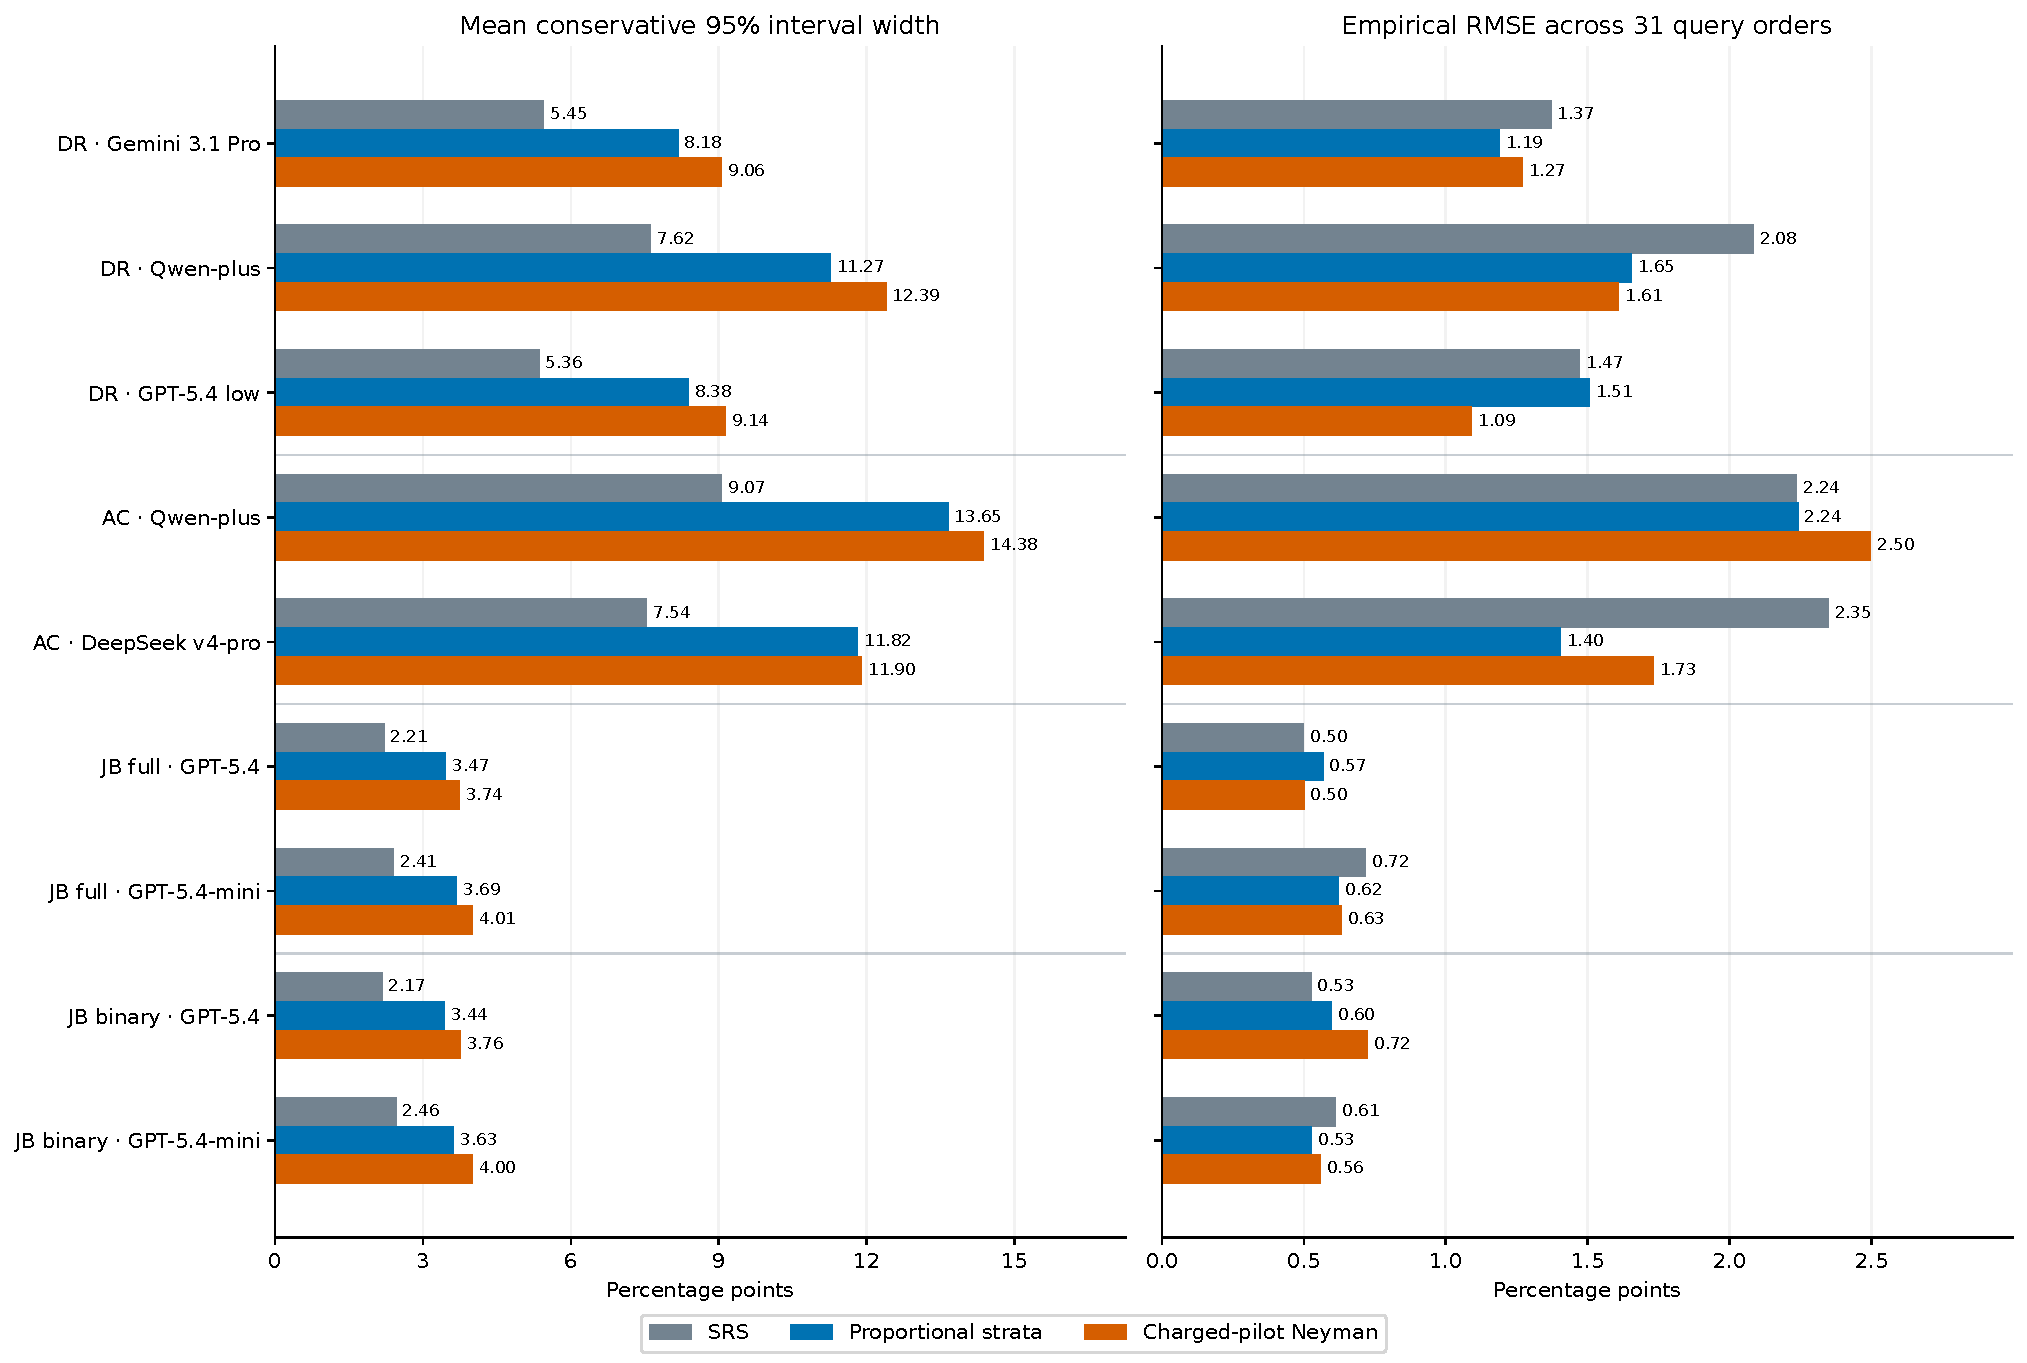
\includegraphics[width=\linewidth,height=0.79\textheight,keepaspectratio]{conjunction_robustness_estimation.pdf}
\caption{Estimation controls at a 20\% criterion budget across all nine cells. Guaranteed interval widths and empirical RMSE are shown separately. The stratified intervals combine finite-population count bounds conservatively; their width alone does not rank point-estimation performance. Pilot labels count toward the same budget. Each empirical quantity summarizes 31 saved orders, while the coverage guarantee follows from the design.}
\label{fig:estimation}
\end{figure}
\FloatBarrier

The released package separates data integrity, scientific replay, and manuscript
validation. Inputs are compact numerical projections with task, output, rater,
criterion and scoring metadata. Original input provenance and content hashes
are in \texttt{data/PROVENANCE.json}; result provenance is stored with the
archived numerical outputs. The following commands run from the repository
root after installing the pinned Python dependencies:
\begin{verbatim}
python -m src.check_package
python -m pytest -q
python -m src.reproduce --mode full --output artifacts/reproduced
python -m src.verify_release --results artifacts/reproduced
python -m src.reproduce_extensions --output artifacts/reproduced-extensions
python -m src.reproduce_extensions --output artifacts/reproduced-extensions --verify-only
python -m src.verify_manuscript_claims --output artifacts/paper-checks/claims.json
python -m src.build_paper
\end{verbatim}
The final command additionally requires Tectonic (tested with version 0.17.0)
and writes a rebuilt PDF separately from the published copy. Initial dependency
installation can require network access; the scientific replay does not call
judge APIs. Rebuilding the PDF can change PDF metadata without changing the
scientific results. The published manuscript includes a claim audit and a
citation audit; the broader technical reading library remains separate from
the selected manuscript bibliography.

Table~\ref{tab:sources} maps the paper's numerical claims to the result groups.
For compactness, paths below are relative to
\texttt{artifacts/expected/}. The executable claim audit records exact row
keys, units, recomputed values and source hashes. It checks selected paper
anchors and accounting identities; the complete scientific reproduction
commands compare the larger archived grids.
\begin{table}[h]
\centering\small
\caption{Numerical source routing for the paper.}
\label{tab:sources}
\begin{tabularx}{\linewidth}{lX}
\toprule
Paper component & Archived source group\\
\midrule
Frames and initial errors & \texttt{conjunction\_policy\_study/study.json} and input tables\\
Query-order curves & \texttt{conjunction\_policy\_study/budget\_curves.csv.gz}\\
Exact expectations and permutations & \texttt{conjunction\_mechanism/}\\
Paired allocation decomposition & \texttt{conjunction\_mechanism/}\\
SRS/mix and whole-task estimates & \texttt{conjunction\_label\_value/}\\
Reference and composition sensitivity & \texttt{conjunction\_robustness/}\\
Stratified estimation controls & \texttt{conjunction\_robustness/}\\
Disclosure endpoints and witnesses & \texttt{information\_disclosure\_replay.json}\\
\bottomrule
\end{tabularx}
\end{table}

\end{document}
